%=========================================================================
% (c) 2011, 2012 Josef Lusticky <xlusti00@stud.fit.vutbr.cz>

\section{Algorithms}
Because of network latency the timestamp received will never be exactly
corresponding to the current time.
One of the main goals of NTP is to deal with the network latency~\cite{ntp-overview}.

As the figure~\ref{fig:ntp-packet} shows and section~\ref{sec:ntp-network} describes,
there are three 64-bit long timestamps in NTP packet: Origin, Receive and Transmit Timestamp.
%The Reference timestamp is when server was synchronised
%! TODO ->
Upon NTP packet arrival, the client determines another timestamp called
Destination Timestamp~\cite{rfc5905}.

Using these four timestamps, NTP client can compute
the local clock offset which is given by $\theta = \frac{1}{2}[(t_2 - t_1) + (t_3 - t_4)]$,
where $t_1$ is the time of the request packet transmission (Origin Timestamp),
$t_2$ is the time of the request packet reception (Receive Timestamp),
$t_3$ is the time of the response packet transmission (Transmit Timestamp) and
$t_4$ is the time of the response packet reception (Destination Timestamp)~\cite{ntp-algor,rfc5905}.

%! figure

%! communication with one server - RFC958
The destination peer calculates the roundtrip delay and clock
      offset relative to the source peer as follows.  Let t1, t2 and t3
      represent the contents of the Originate Timestamp, Receive
      Timestamp and Transmit Timestamp fields and t4 the local time the
      NTP message is received.  Then the roundtrip delay d and clock
      offset c is:

         d = (t4 - t1) - (t3 - t2)  and  c = (t2 - t1 + t3 - t4)/2 .

      The implicit assumption in the above is that the one-way delay is
      statistically half the roundtrip delay and that the intrinsic
      drift rates of both the client and server clocks are small and
      close to the same value.
%one server

When computing result from more servers the intersection algorithms is used
for selecting the possible most exact timestamp received from various servers~\cite{rfc5905}.
% Derived from Murzollo algorithm but the base remains... ~\cite{ntp-history}.
The resulting exact timestamp does not have to be the same
as one of those servers provided.
First of all a set of bad and good servers must be made.
Bad servers are called Falsetickers and good are called Truechimers~\cite{rfc5905}.
The division to these sets is based on their response.
As one can assume for sensible result there must be more Truechimers than Falsetickers~\cite{rfc5905}.

Intersection algorithm computes with estimates converted to intervals.
Figure~\ref{fig:ntp-intersection} shows the computation for the following example:
If we have the estimates $10 \pm 2$, $12 \pm 1$ and $11 \pm 1$
then these intervals are $<8; 12>$, $<11; 13>$ and $<10; 12>$ which
intersect to form $<11; 12>$ or $11.5 \pm 0.5$ as consistent with all three values.
The arithmetic mean is used as a value of result.
When querying servers again, the algorithm repeats but the new result computation
also depends on the previous result~\cite{rfc5905}.
This eliminates possible jitter which can be caused by repeatedly querying the servers
and getting slightly different answers from them.

\begin{figure}
	\centering
	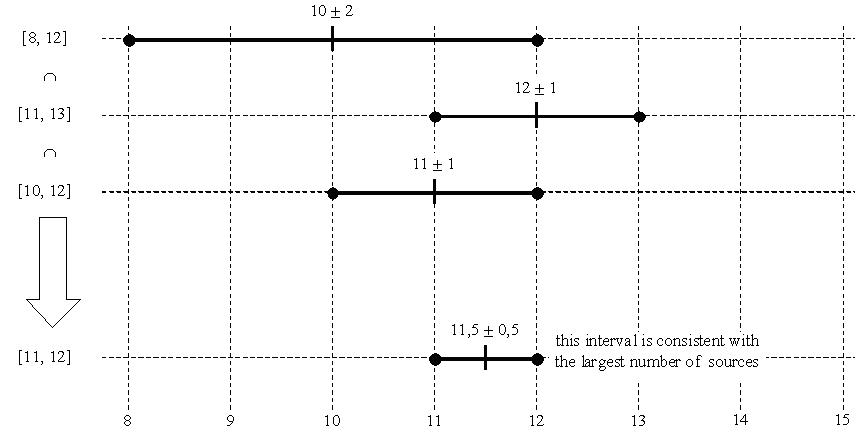
\includegraphics[width=13cm,keepaspectratio]{fig/Marzullo_example-1.jpg}
	\caption{Intersection algorithm by D. Exb}
	\label{fig:ntp-intersection}
	\bigskip
\end{figure}

%Since the clients complying with a subset of NTP, called
%the Simple Network Time Protocol (SNTPv4) [RFC4330], do not need to
%implement the mitigation algorithms ... ~\cite{rfc5905}.
